% !TEX root = ../../main.tex

\subsection{Thermogravimetry results}

From the TGA curve of the pristine UiO-66 material, 
it is immediately obvious that there are some defects 
already present in the sample. By using the normalized
mass at \SI{420}{\degreeCelsius} a linker-to-cluster 
ratio of around 11:1 can be calculated. This corresponds 
to one BDC linker per cluster on average and shows that
there are still intrinsic defects in the as-synthesised 
structure.

The graphs in \autoref{def:fgr:tga-defects} summarize the 
trends in missing linker defects as calculated through 
thermogravimetry with all the samples used.

When DMF is used as a solvent, the resulting leached samples 
have a 

Since multiple concentrations of modulator were used only with 
DMF, inly a general trend is available.


\begin{figure}[htb]
    \centering

    \begin{subfigure}{0.45\linewidth}
        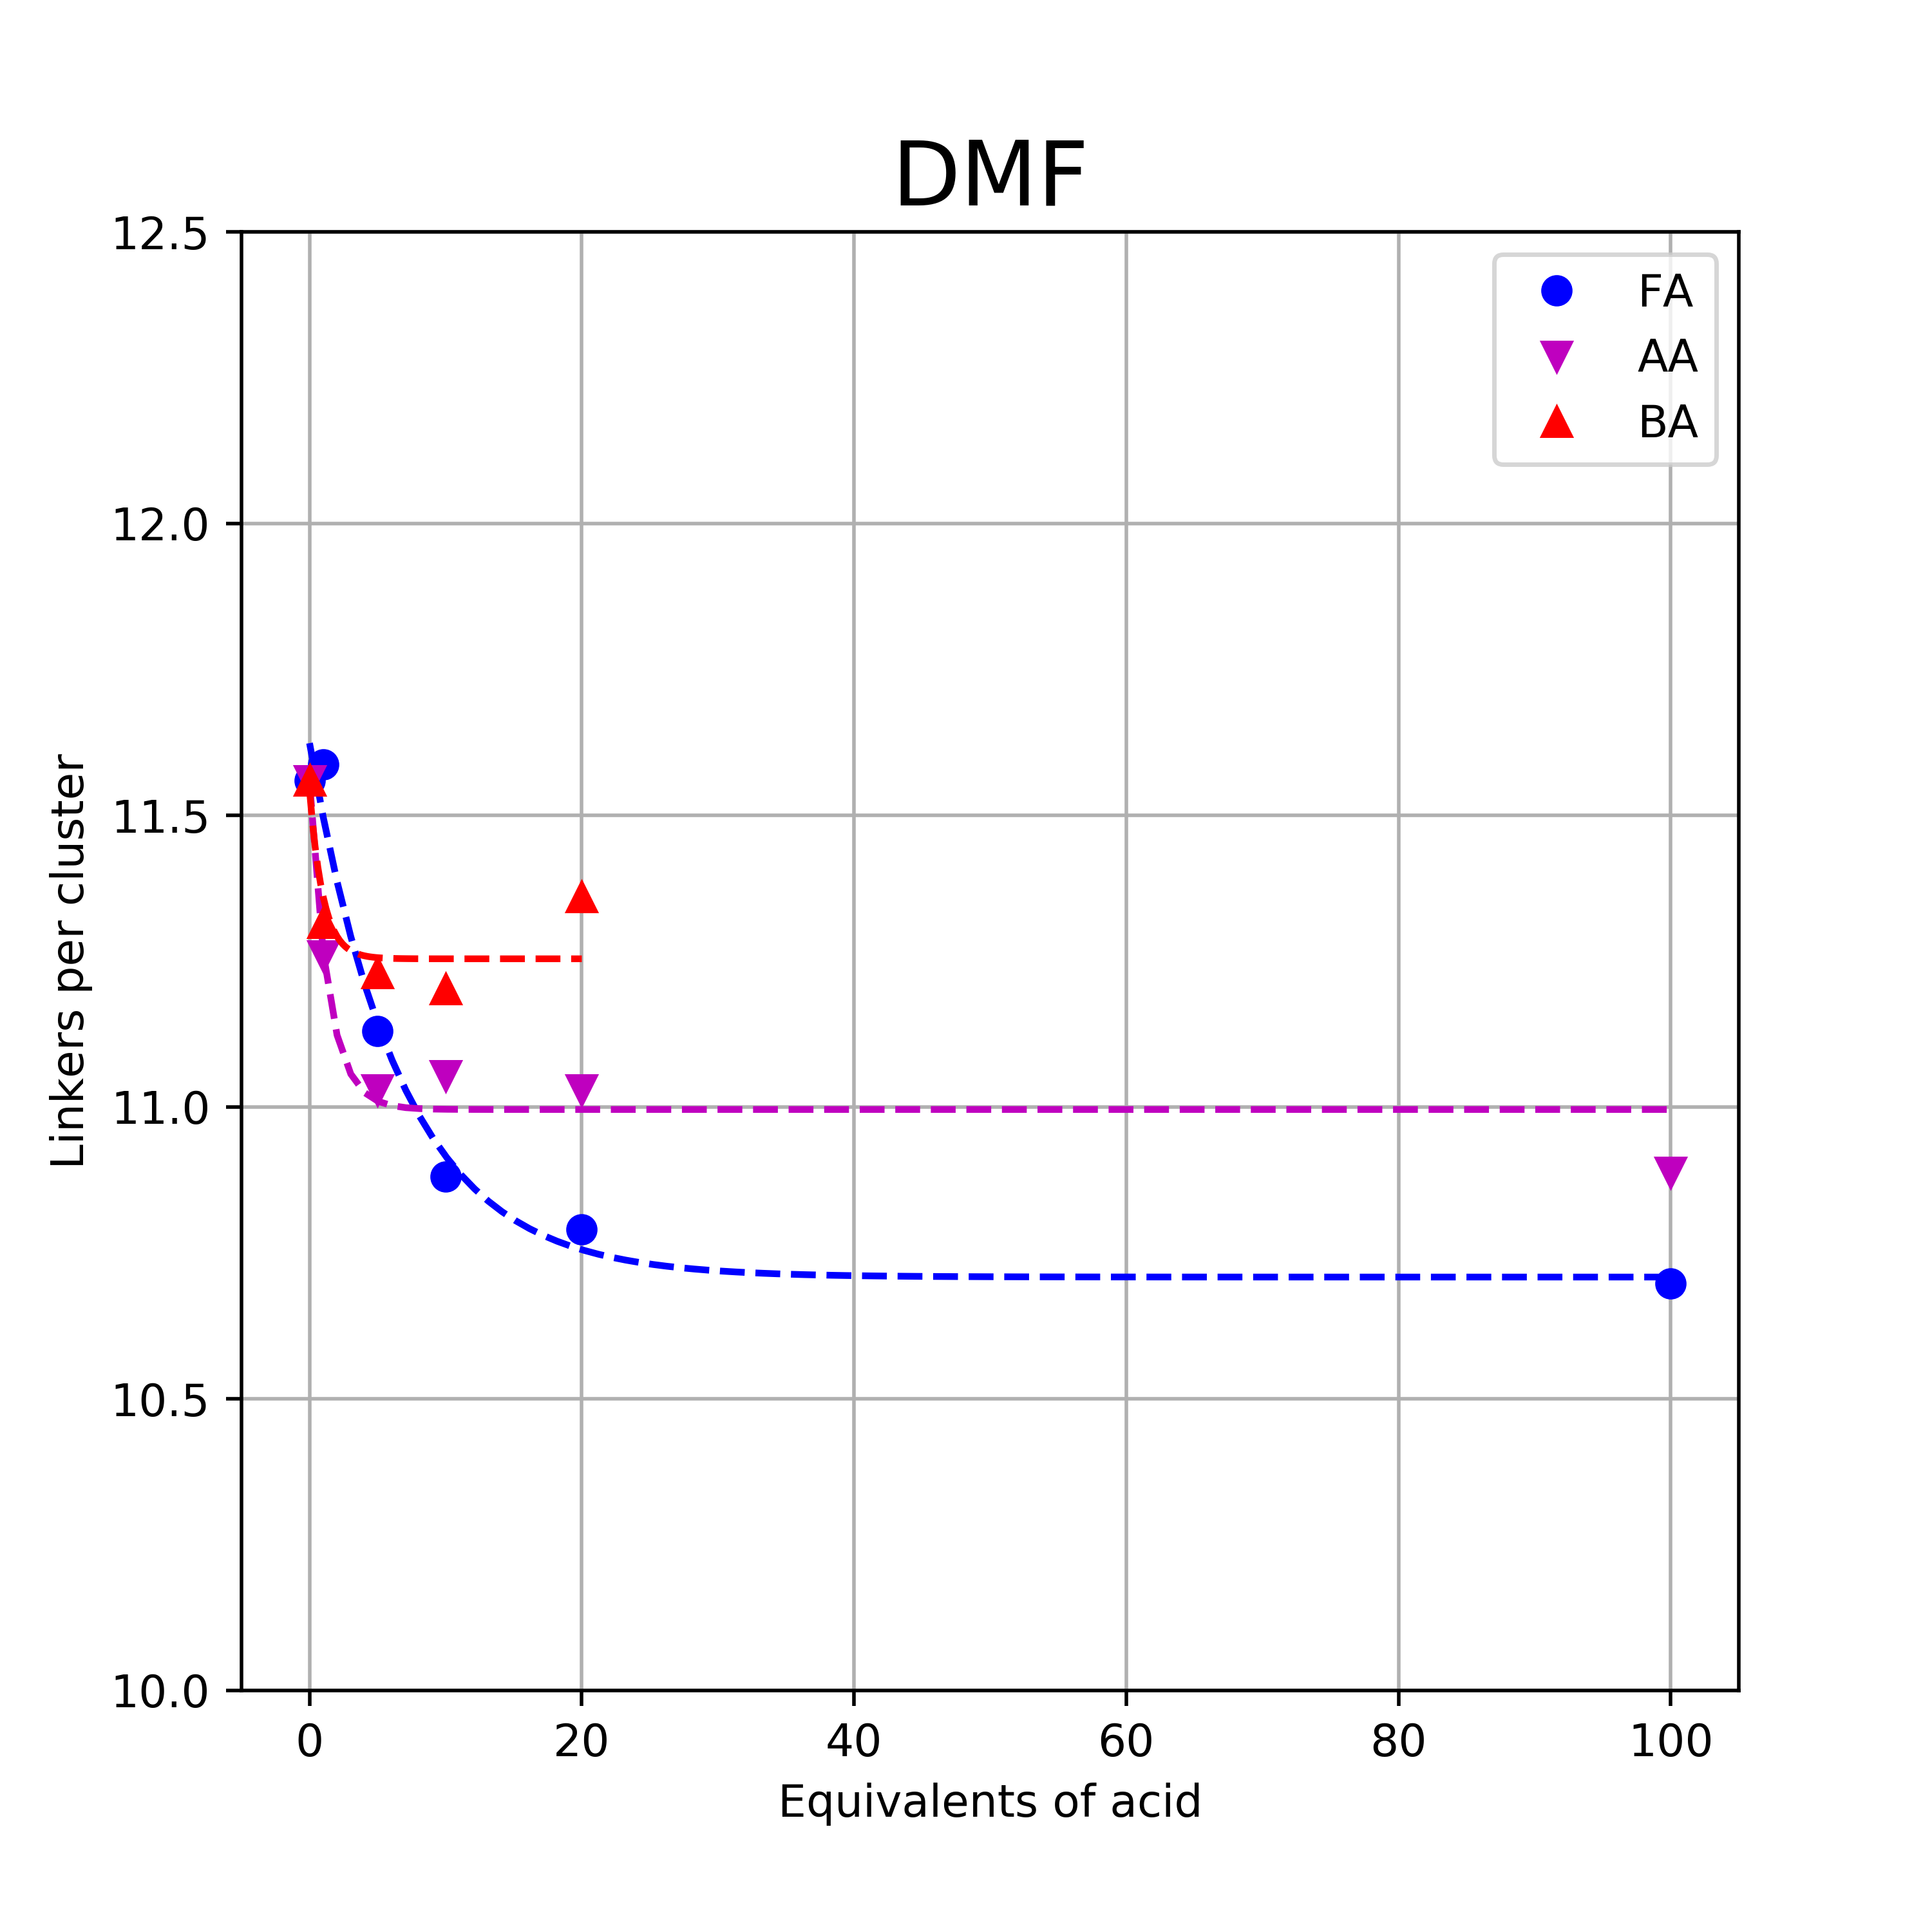
\includegraphics[width=\textwidth]{tga/DMF-def-overview}%
        \label{def:fgr:tga-dmf-linkers}
    \end{subfigure}
    \begin{subfigure}{0.45\linewidth}
        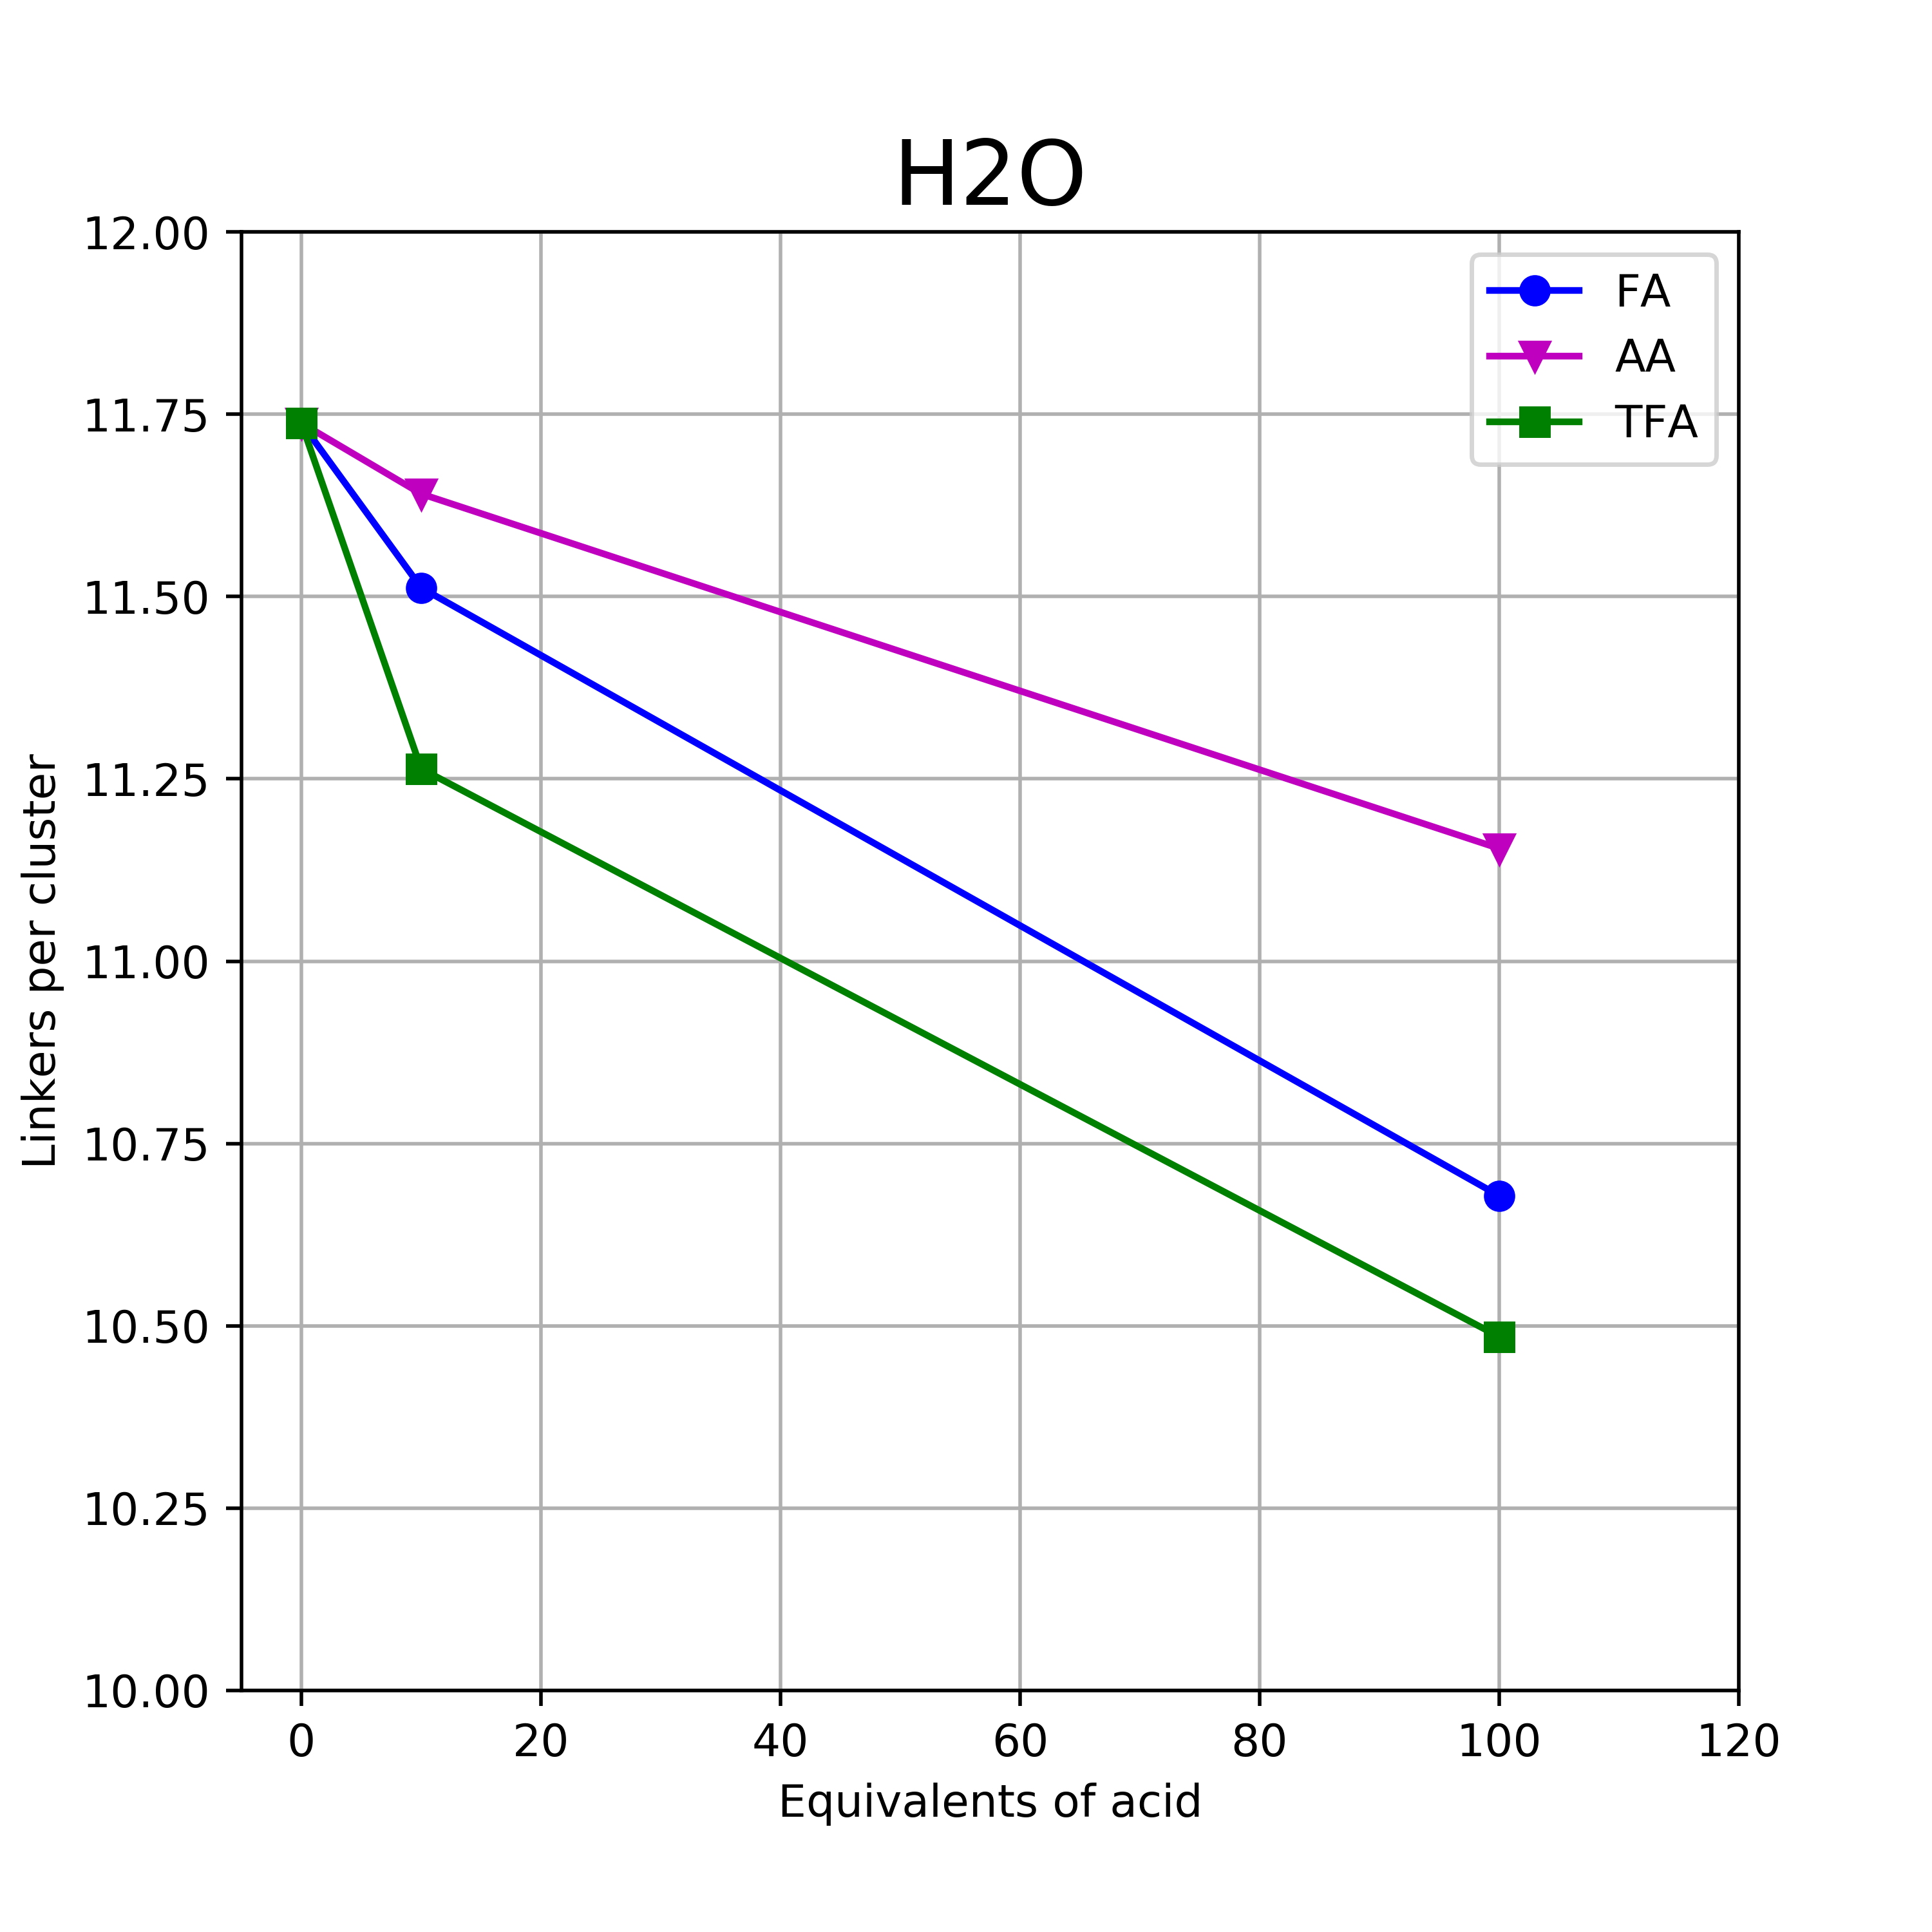
\includegraphics[width=\textwidth]{tga/H2O-def-overview}%
        \label{def:fgr:tga-h2o-linkers}
    \end{subfigure}

    
    \begin{subfigure}{0.45\linewidth}
        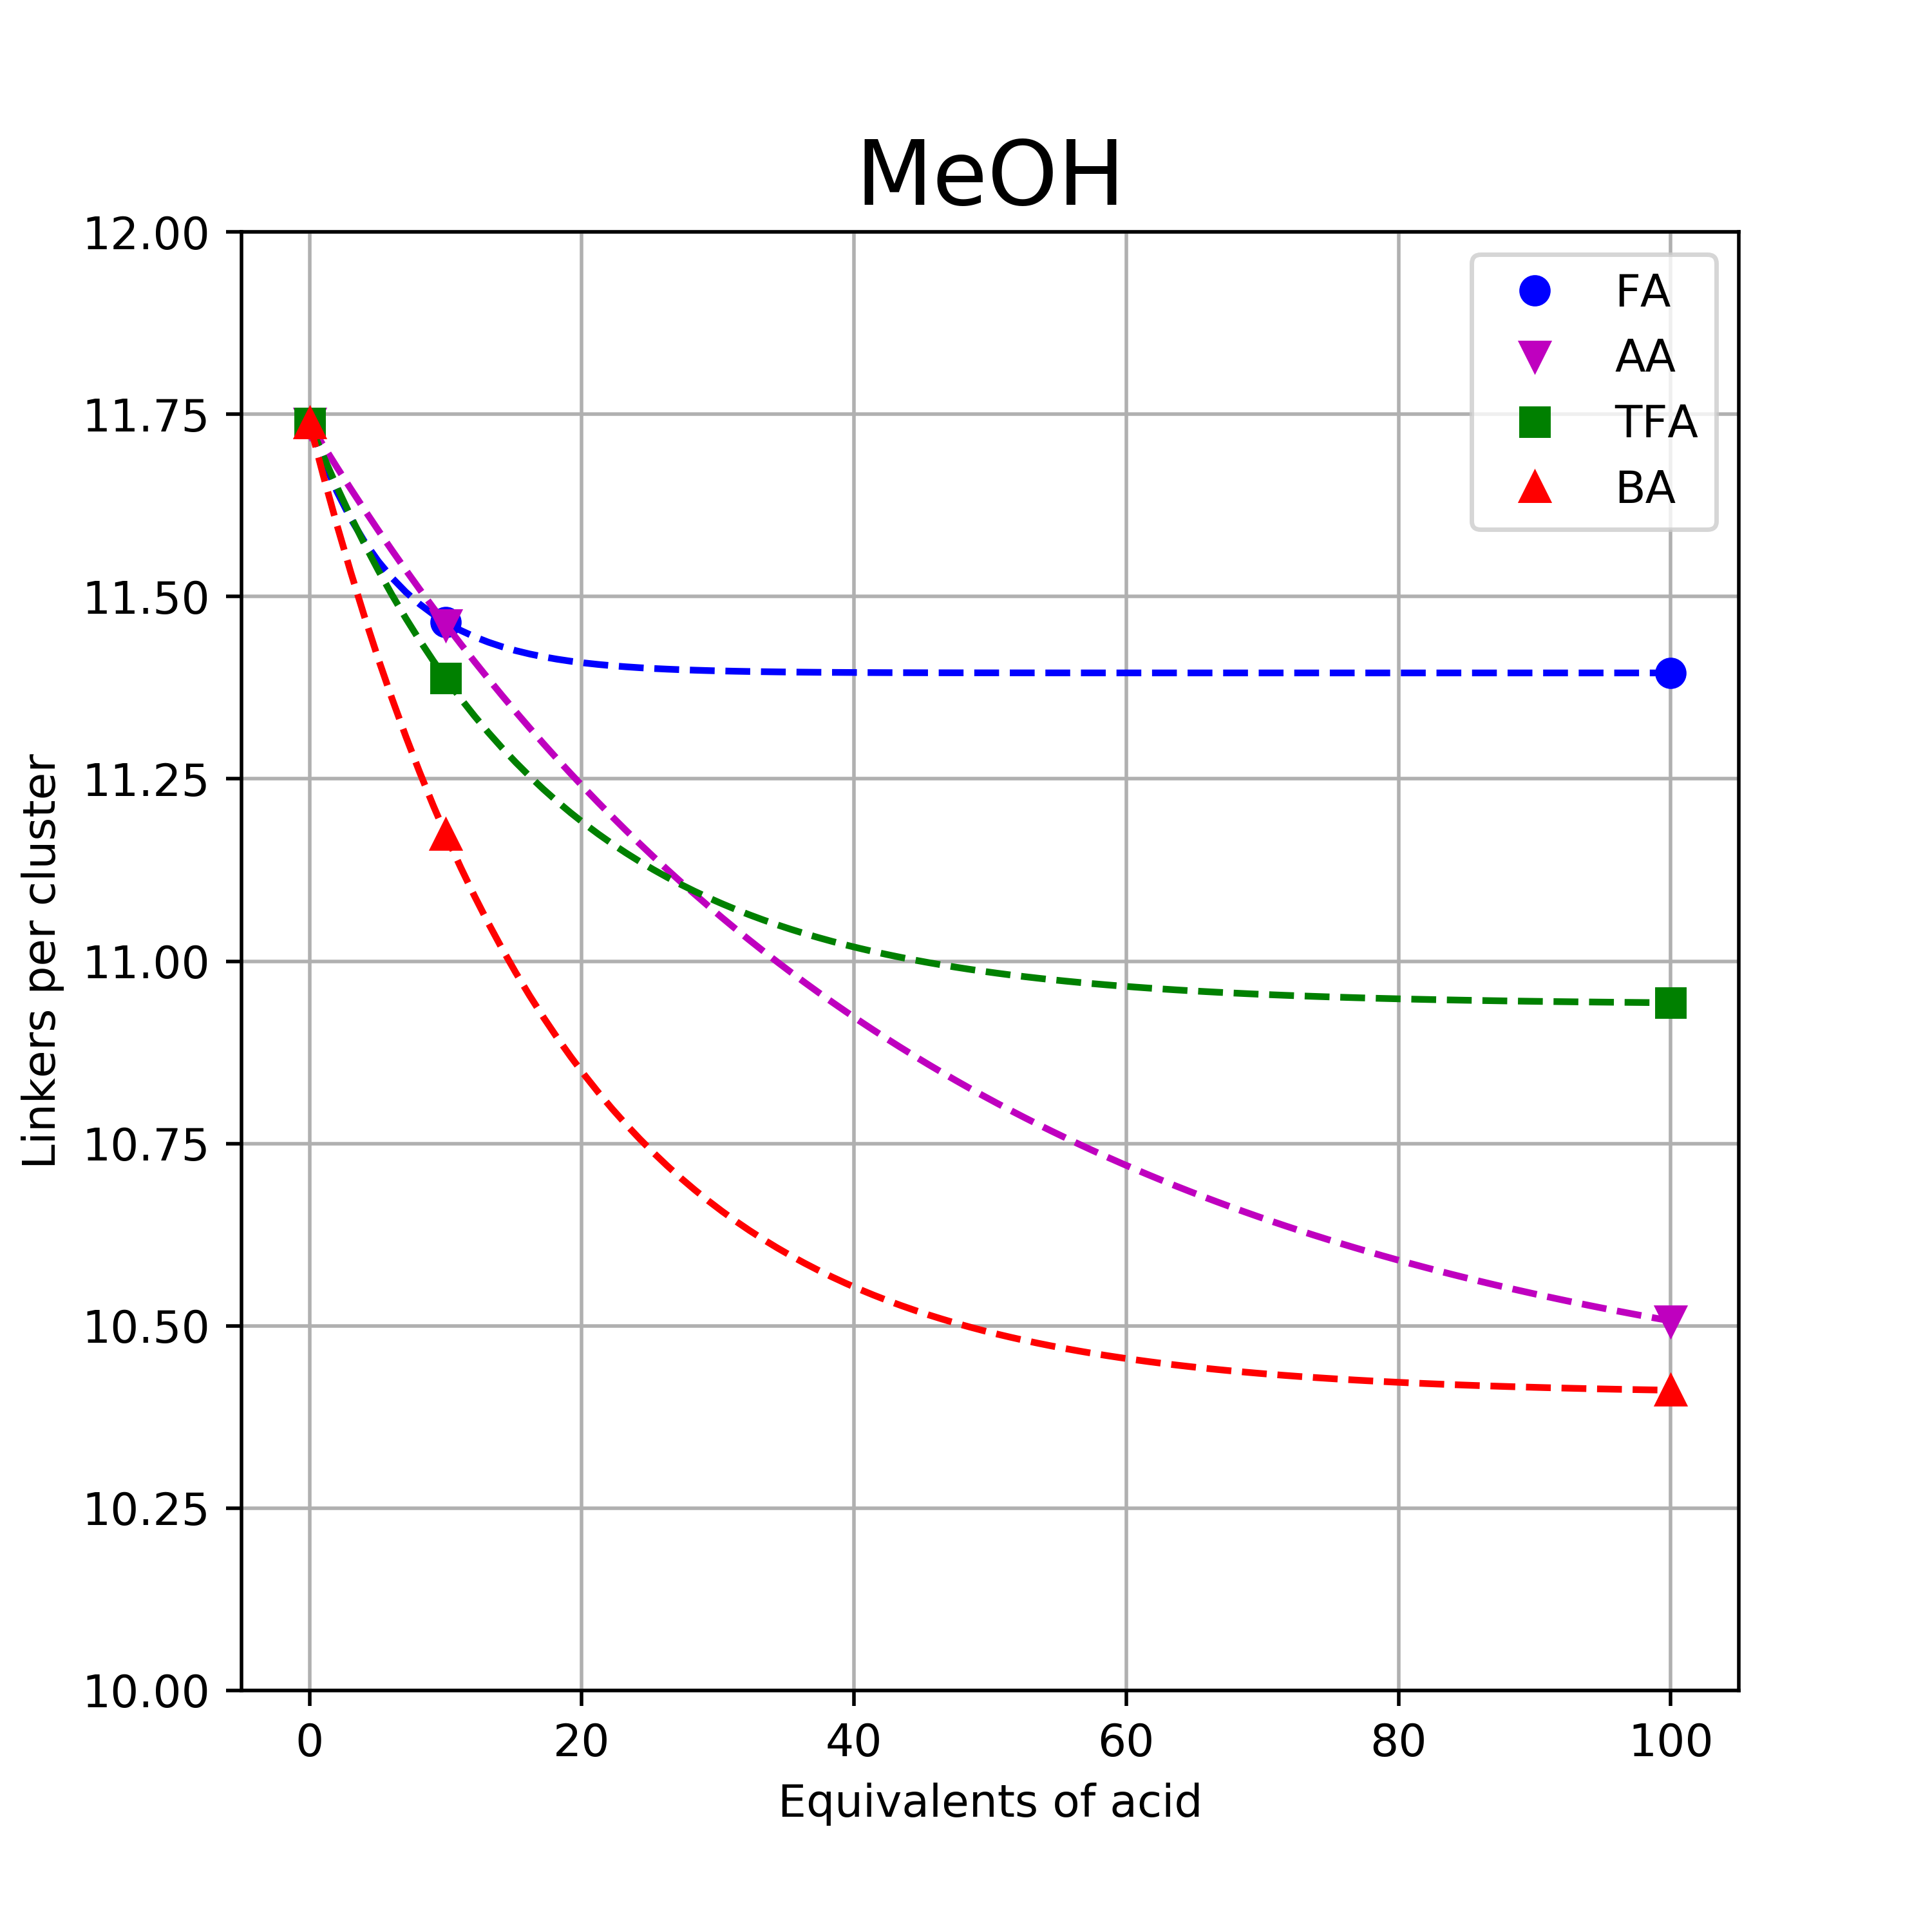
\includegraphics[width=\textwidth]{tga/MeOH-def-overview}%
        \label{def:fgr:tga-meoh-linkers}
    \end{subfigure}
    \begin{subfigure}{0.45\linewidth}
        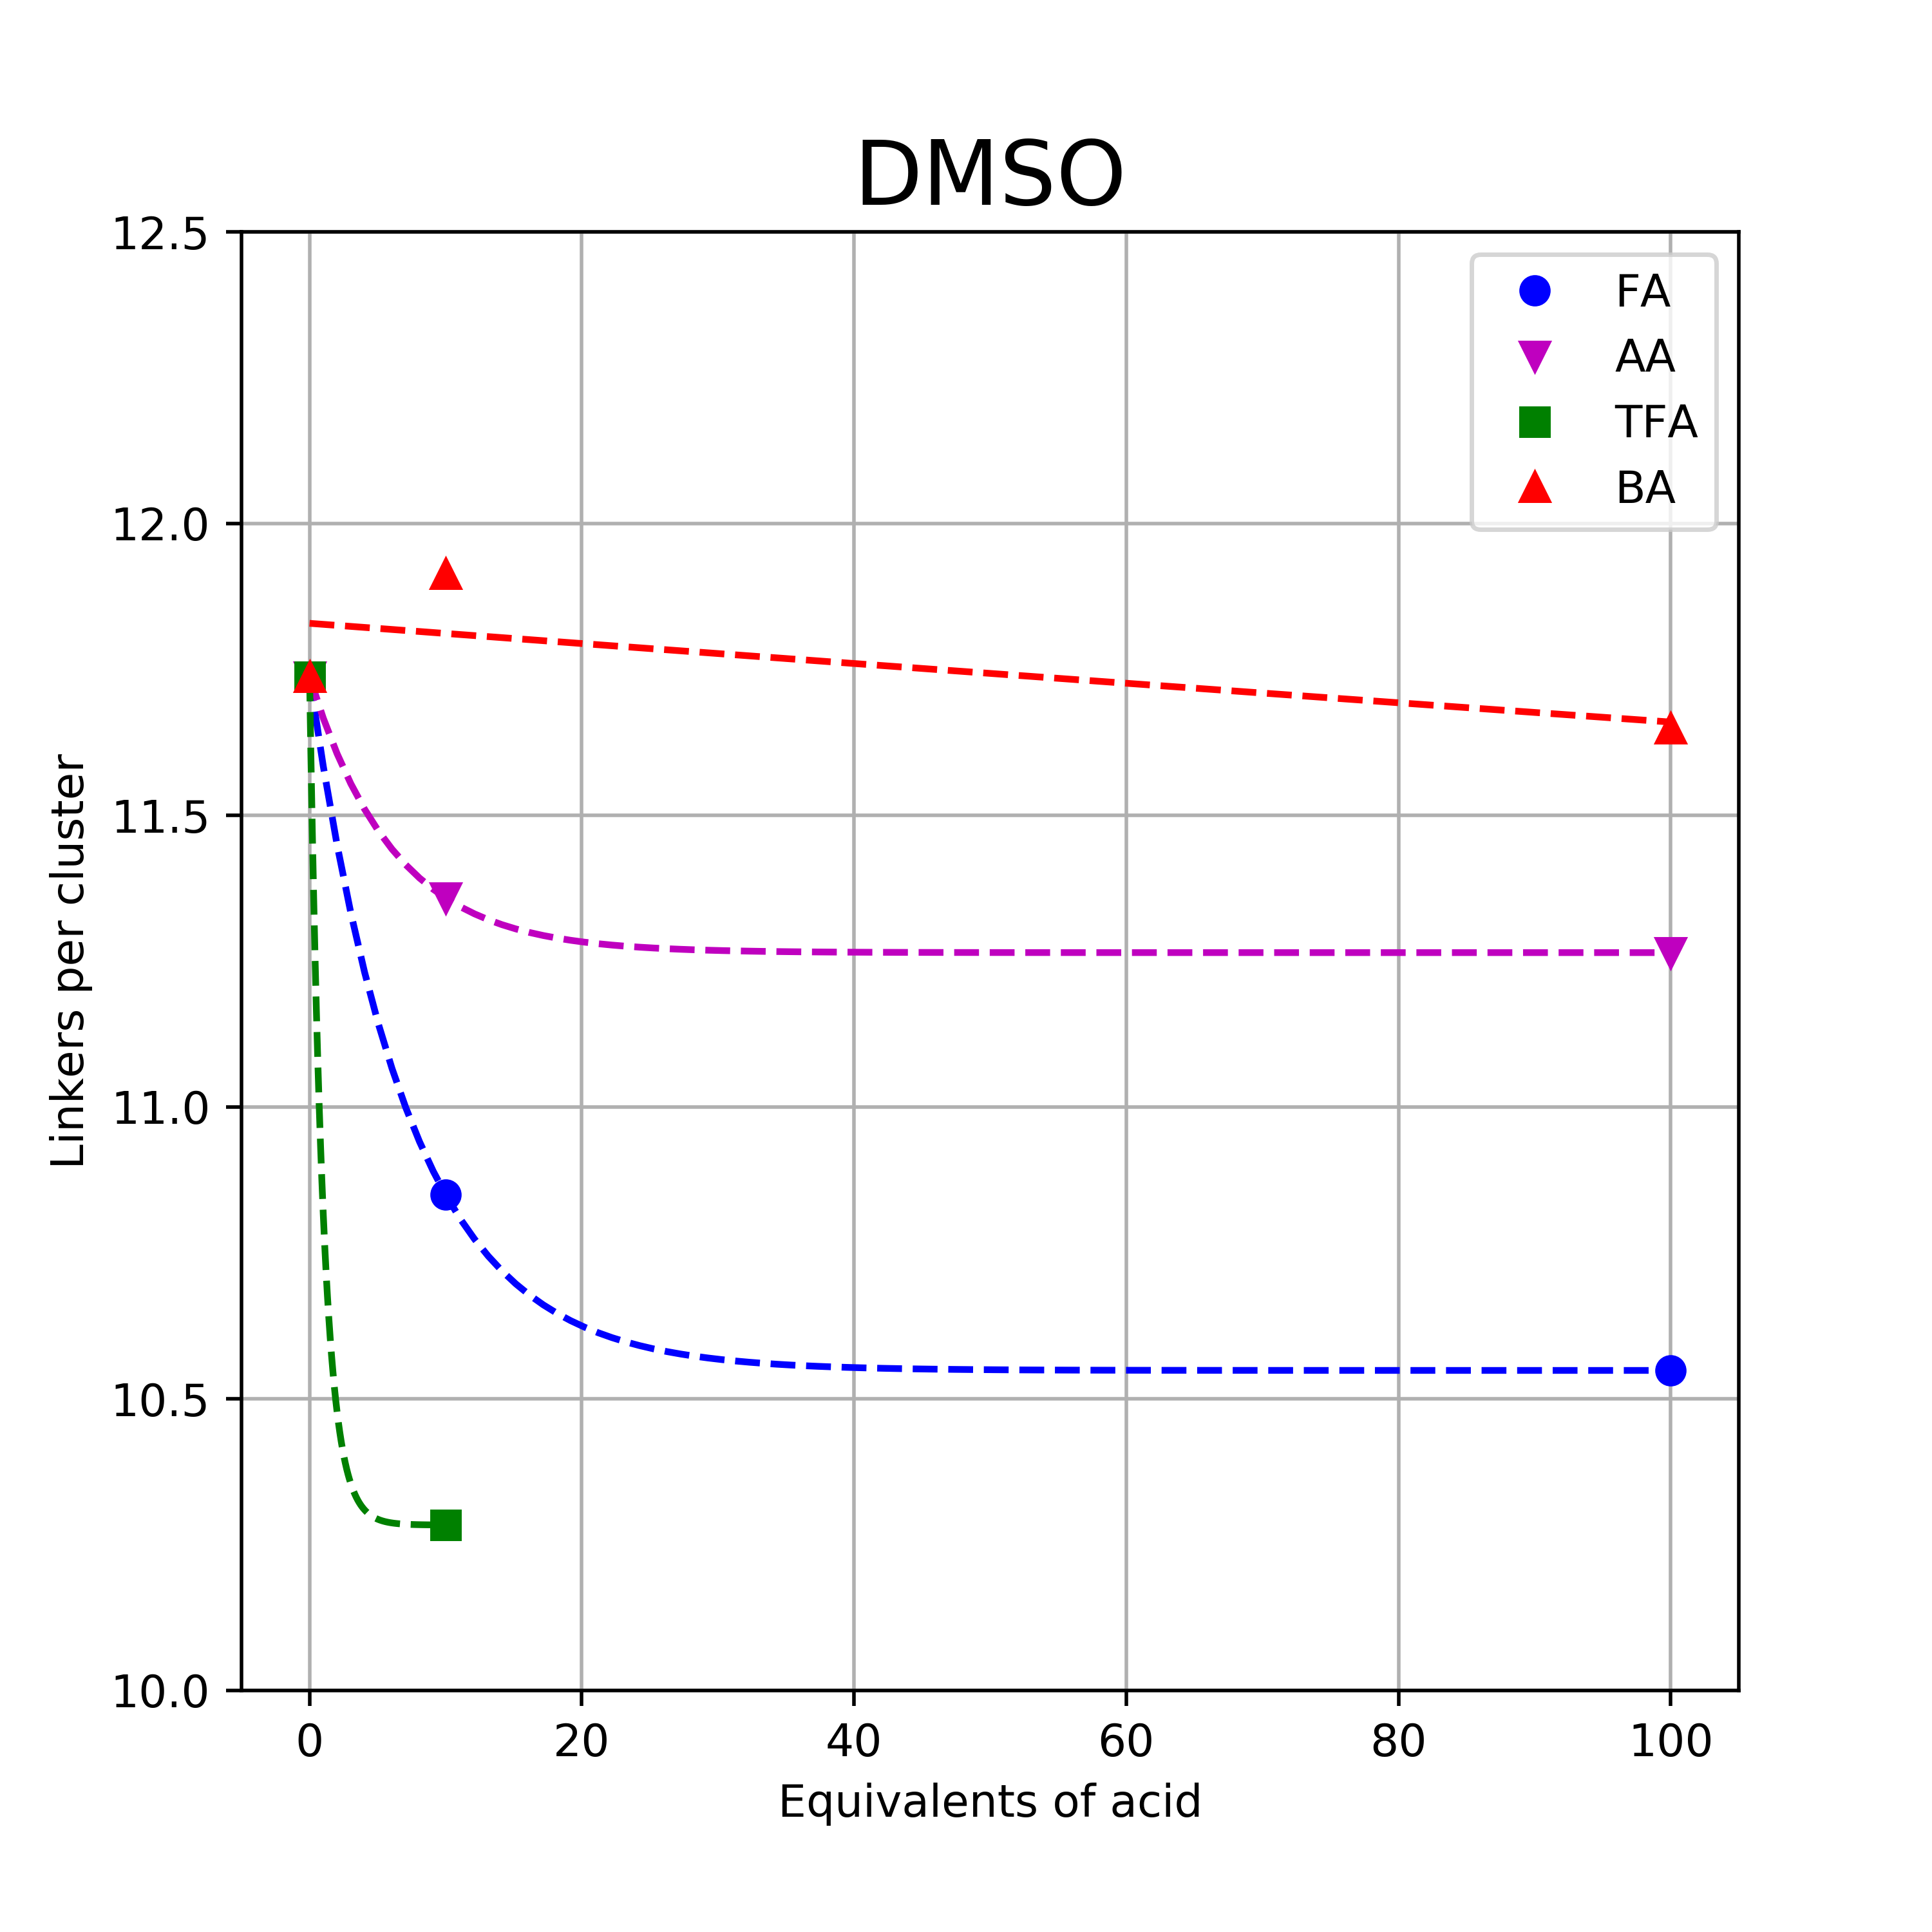
\includegraphics[width=\textwidth]{tga/DMSO-def-overview}%
        \label{def:fgr:tga-dmso-linkers}
    \end{subfigure}

    \caption{Calculated linker-to-node ratio from the TGA curve 
    normalized mass at \SI{420}{\degreeCelsius} for (a) DMF 
    (b) \ce{H2O}, (c) \ce{MeOH} and (d) DMSO leached samples.
    A ratio of 12 to 1 corresponds to a completely defect-free
    structure.}%
    \label{def:fgr:tga-defects}
    
\end{figure}
